% Semantic Afterlife manuscript (Stage 7).
% Every quantitative claim carries a same-line LaTeX comment: artifact path + run_id.
% Cite only VERIFIED entries in docs/literature/related-work.md (see paper/refs.bib).
% Do not treat this file as a filled 50-paper.mdc table of contents: MSM, half-life,
% currents, and cross-model basins were not established (S3/S4/S5/S6).
\documentclass[11pt,a4paper]{article}

\usepackage[T1]{fontenc}
\usepackage[utf8]{inputenc}
\usepackage{lmodern}
\usepackage[margin=1in]{geometry}
\usepackage{graphicx}
\usepackage{booktabs}
\usepackage{amsmath}
\usepackage{amssymb}
\usepackage{natbib}
\usepackage[hidelinks]{hyperref}
\usepackage{setspace}
\usepackage{microtype}

\graphicspath{{../artifacts/}}
\setstretch{1.08}

\title{Semantic Afterlife:\\
Lock Occupancy After the Prompt Leaves the Window}
\author{Adam Cage}
\date{}

\begin{document}
\maketitle

\begin{abstract}
A language model whose input is truncated to the last $W$ generated tokens
continues after the original prompt has left that window. We ask what remains
in the trajectory: a unique stationary law, a temperature-robust cycle, a
domain-tagged lock, or diffusion. The object is the \emph{afterlife}: the
segment after seed eviction, not the prompt-conditioned transient.

On one instruct generator (\texttt{or-qwen3-8b}) under a re-prompt protocol
(P1), a textual fixed-point lock is the typical $T{=}0.3$ outcome through
twelve turnovers of $W{=}4096$. % artifacts/stage-5/occupancy/lock_rate_by_seed.csv @ s5-lock-occupancy-20260905T164327Z-6780902f
Last-band occupancy retains an ensemble domain gap (F4 distinguishability);
that gap is not recovered prompt memory (H2). % artifacts/stage-6/occupancy/domain_separation_last_band.csv @ s6-embed-third-space-20260906T082301Z-588eff8f
That occupancy result is a subsection, not
the title claim: the third space is an NHST whisker, not architecture-independent
robustness. % artifacts/stage-6/occupancy/domain_separation_last_band.csv @ s6-embed-third-space-20260906T082301Z-588eff8f
The lock is not universal across hosted generators, is absent at
$T{=}1.5$ for $W{=}4096$ on this model, and is not a validated Markov state model. % artifacts/stage-4/grid/looping_rate_by_cell.csv @ s4-w4096-new-temps-20260904T103121Z-589c8eb1
We did not measure a sliding native KV cache. Degeneracy is the sample, not a
filter that was applied and then forgotten. % artifacts/stage-5/occupancy/lock_rate_by_seed.csv @ s5-degeneracy-20260906T030145Z-deb4c3bd
\end{abstract}

\section{Introduction}
\label{sec:intro}

Let $X_t \in V^W$ be the last $W$ generator tokens, $Y_t \sim P_\theta(\cdot \mid X_t)$,
and $X_{t+1} = \mathrm{Tail}_W(X_t \oplus Y_t)$. After roughly one window of
generated tokens the seed is physically absent from the model's input. Call
that eviction the \emph{horizon}, and the subsequent trajectory the
\emph{afterlife}. The scientific question is not whether a model can follow a
prompt while the prompt is present. It is whether, after eviction, the
trajectory retains seed identity, collapses onto a model-specific lock, or
diffuses.

That question is easy to answer wrongly. A looping trajectory occupies one
point in representation space and reports a confined mean-squared displacement
for reasons that have nothing to do with semantics. This project recorded that
error once and does not repeat it: degeneracy is labelled before geometry is
read, and a looping row is not sold as a confined basin.

The experiments that exist are Stages~0--6 of a pre-registered plan
(\texttt{docs/research-plan.md}). Stage~3 asked for metastable semantic states
via VAMP/PCCA+ and did not obtain a validated MSM. % artifacts/stage-3/dynamics/k_stability.md @ s3-dynamics-20260901T204521Z-f21d5908
Stage~4 asked for a
temperature window of non-looping confined motion (H5) and did not find it. % artifacts/stage-4/grid/clean_alpha_by_cell.csv @ s4-w4096-new-temps-20260904T103121Z-589c8eb1
Stage~5--6 asked whether, \emph{given} the lock, last-band occupancy still
shows an ensemble domain gap and whether replica pairs collapse. The
last-band result is distinguishability, not recovered prompt memory (H2).
Sign agreement holds in three embedding spaces on this generator,
protocol, and temperature; the third space is an NHST whisker, not
architecture-independent robustness. % artifacts/stage-6/occupancy/domain_separation_last_band.csv @ s6-embed-third-space-20260906T082301Z-588eff8f
They do not establish H1, H5, or a result for language models as
a class.

Section~\ref{sec:related} places the afterlife against verified related work.
Section~\ref{sec:protocol} defines P1, the cost law, degeneracy, and the two
occupancy tests used later. Section~\ref{sec:results} reports stages in the
order they were run. Section~\ref{sec:limitations} lists what the design cannot
establish. Section~\ref{sec:discussion} separates established claims from
parked ones.

\section{Related work}
\label{sec:related}

We cite only sources marked VERIFIED in the project literature log.
Unverified items are not used as support.

\citet{zekri2024} study autoregressive generation as a Markov chain on the
context and, under contraction of the next-token kernel in total variation,
prove existence of a unique stationary distribution together with exponential
mixing. That theorem is the right null for a \emph{unique} long-run law. It is
not a measurement of whether our trajectories occupy one lock or several
domain-tagged locks, and it does not replace an occupancy test after eviction.

\citet{wang2025} report decoding cycles that remain under temperature sampling,
and treat repetition as a dynamical regime rather than a decoding bug. Our
Stage~2 comparison is the opposite direction on the model axis: at $T{=}0.3$,
\texttt{or-gemma-4-31b} produced $0/8$ textual fixed points while % artifacts/stage-2/model-axis/rates/fixed_point_rates.csv @ s2-rates-20260901T125506Z-41d2e88e
\texttt{or-gpt-oss-120b} produced $8/8$ (Section~\ref{sec:s2}). % artifacts/stage-2/model-axis/rates/fixed_point_rates.csv @ s2-rates-20260901T125506Z-41d2e88e
Cycle robustness
to temperature in their setting is not a licence to call our lock
temperature-universal; Stage~4 already falsifies that reading on
\texttt{or-qwen3-8b} at $T{=}1.5$, $W{=}4096$. % artifacts/stage-4/grid/looping_rate_by_cell.csv @ s4-w4096-new-temps-20260904T103121Z-589c8eb1

\citet{geng2026} argue that raising temperature lengthens transients before a
stable regime. Stage~4 is consistent with a later onset of non-looping
behaviour at $T{=}1.5$, but that stage did not estimate a mixing time, and the % artifacts/stage-4/grid/clean_alpha_by_cell.csv @ s4-w4096-new-temps-20260904T103121Z-589c8eb1
non-looping rows are subdiffusive rather than a validated stationary sample. % artifacts/stage-4/grid/clean_alpha_by_cell.csv @ s4-w4096-new-temps-20260904T103121Z-589c8eb1

\citet{ko2026} describe interlocutor-conditioned attractors in multi-agent
dialogue. Our protocol has no interlocutor. A lock that appears without a
second speaker is a different object; we do not import their attractor language
as a finding about our trajectories.

\citet{chen2026horizon} separate horizon, context, and memory as distinct axes.
We impose $W$ by truncation (P1) and begin the scientific object after the seed
has left that window. That is the intended delta relative to prompt-conditioned
long-context work: the afterlife is not another name for in-window reasoning.

Markov-state and VAMP methodology from molecular dynamics
\citep{wu2020vampnets,paul2019core} is the toolkit Stage~3 applied to
embeddings. The toolkit is not the result. Stage~3 did not validate an MSM on
these trajectories (Section~\ref{sec:s3}). % artifacts/stage-3/dynamics/k_stability.md @ s3-dynamics-20260901T204521Z-f21d5908

\section{Protocol}
\label{sec:protocol}

\subsection{Generator, window, and P1}
\label{sec:p1}

All occupancy numbers in Sections~\ref{sec:s5}--\ref{sec:s6} use
\texttt{or-qwen3-8b} (Qwen3-8B-Instruct via OpenRouter; served provider
\texttt{Alibaba} on every completed occupancy step), $W{=}4096$,
$T{=}0.3$, block $B{=}512$, analysis chunks of $1024$ generator tokens, % docs/stages/stage-5/REPORT.md @ s5-lock-occupancy-20260905T164327Z-6780902f
non-overlapping, and twelve turnovers of $W$ after the seed. % docs/stages/stage-5/REPORT.md @ s5-lock-occupancy-20260905T164327Z-6780902f
The continuation mechanism is \texttt{raw\_completion}, not
\texttt{assistant\_prefill} and not \texttt{chat\_instructed}. Protocol P1
is the re-prompt: the last $W$ tokens of generated text are re-encoded and
sent as a new prompt. P1 and the continuation mechanism are distinct axes
(glossary). Stage~2 already measured a prefill-versus-raw arm on this
generator; occupancy does not reuse that arm as its protocol.
The input construction is not a sliding native KV cache. The
gap is named in Section~\ref{sec:limitations} and parked in ADR-0017; it is
not treated as measured.

A \emph{turnover} is $T/W$ in generator tokens. The \emph{horizon} is the
step at which the seed has fully left the window. Last-band occupancy uses
the final complete turnover band, not a mean over the whole trajectory.

\subsection{Cost law}
\label{sec:cost}

Hosted spend follows the recorded ledger, not a model card. Stage~0 capability
audit cost $\$0.0128$. % docs/stages/stage-0/REPORT.md @ s0 audit
Stage~1
generation billed $\$6.32$ on % docs/stages/stage-1/REPORT.md @ s1-pilot-core-20260830T134147Z-f1cce9ec
\texttt{s1-pilot-core-20260830T134147Z-f1cce9ec}. % docs/stages/stage-1/REPORT.md @ s1-pilot-core-20260830T134147Z-f1cce9ec
Stage~4 hosted generation
billed $\$3.4383$ % docs/stages/stage-4/REPORT.md @ s4-w4096-new-temps-20260904T103121Z-589c8eb1
(\texttt{s4-w4096-new-temps-20260904T103121Z-589c8eb1},
\texttt{s4-w8192-20260904T120057Z-ce82ce55}). % docs/stages/stage-4/REPORT.md @ s4-w4096-new-temps-20260904T103121Z-589c8eb1
Stage~5 generation billed
$\$1.3385$ (\texttt{s5-lock-occupancy-20260905T164327Z-6780902f}). % docs/stages/stage-5/REPORT.md @ s5-lock-occupancy-20260905T164327Z-6780902f
Stage~6 used cached Gemini embeddings at hosted $\$0$. % docs/stages/stage-6/REPORT.md @ s6-embed-third-space-20260906T082301Z-588eff8f
Project hosted spend
at Stage~6 close was $\$16.34$ of a $\$200$ ceiling. % docs/stages/stage-6/REPORT.md @ ledger
No Stage~7 generation or embedding was run.

\subsection{Degeneracy is the sample}
\label{sec:degeneracy}

A trajectory is labelled a textual fixed point when calibrated repetition
statistics cross a threshold derived from a human-prose reference corpus:
mean $3$-gram Jaccard $0.083$ and late-window Jaccard $0.0122$. % artifacts/stage-1/degeneracy/degeneracy_verdicts.meta.json @ s1-degeneracy-20260831T070038Z-b2f6f0c9
Those two numbers are not retuned in this manuscript.

On the Stage~5--6 occupancy panel, $19/20$ domain trajectories and $1/2$ love % artifacts/stage-5/occupancy/lock_rate_by_seed.csv @ s5-lock-occupancy-20260905T164327Z-6780902f
trajectories meet the lock rule; $10/10$ domain seeds have at least one lock. % artifacts/stage-5/occupancy/lock_rate_by_seed.csv @ s5-lock-occupancy-20260905T164327Z-6780902f
Occupancy is therefore a statement about locked trajectories, not about a
clean non-looping subsample. Geometry on a looping row is not interpreted as
a confined semantic basin. Love is one of the ten F4 domain seeds, not a
held-out class.

\subsection{Occupancy tests F4 and F6}
\label{sec:f4f6}

Let $D_{\mathrm{within}}$ be the mean cosine distance among last-band
centroids of trajectories that share a seed domain, and $D_{\mathrm{between}}$
the mean cosine distance among last-band centroids from different domains.
The domain gap is $\Delta_{\mathrm{dom}} = D_{\mathrm{between}} - D_{\mathrm{within}}$.
Domains are \emph{separated} when the bootstrap 95\% CI for % docs/stages/stage-5/PLAN.md @ s5-lock-occupancy-20260905T164327Z-6780902f
$\Delta_{\mathrm{dom}}$ excludes $0$ from above. % docs/stages/stage-5/PLAN.md @ s5-lock-occupancy-20260905T164327Z-6780902f

For each matched replica pair, $\Delta_{\mathrm{pair}}(t)$ is the cosine
distance between the two centroids in turnover band $t$, minus the same
quantity in band $0$. The pair is operationally \emph{collapsed} when the % docs/stages/stage-6/REPORT.md @ s6-embed-third-space-20260906T082301Z-588eff8f
last-band CI for $\Delta_{\mathrm{pair}}$ includes $0$. That operational % docs/stages/stage-6/REPORT.md @ s6-embed-third-space-20260906T082301Z-588eff8f
definition is not occupancy of one shared lock: a CI that includes $0$ can % docs/stages/stage-6/REPORT.md @ s6-embed-third-space-20260906T082301Z-588eff8f
be an underpowered non-detection, and a last-band matrix can still show
two within-seed diagonals. % docs/stages/stage-6/REPORT.md @ s6-embed-third-space-20260906T082301Z-588eff8f

F4 and F6 are assembled from occupancy sidecars
(\texttt{scripts/assemble\_stage6\_occupancy.py}), not from a CLI
\texttt{analyze separation} pass and not from a twins table with
\texttt{scope=all}.

\section{Results}
\label{sec:results}

\subsection{Stage 0: the representation stack exists; hosted bases do not}
\label{sec:s0}

Three embedding endpoints accepted the audit texts, returned the advertised
widths, and L2-normalised: \texttt{bge-m3} ($1024$), % artifacts/stage-0/audit/s0_embeddings.csv @ s0 audit
\texttt{qwen3-embed-8b} ($4096$), \texttt{gemini-embed-001} ($3072$). % artifacts/stage-0/audit/s0_embeddings.csv @ s0 audit
No hosted \emph{base} (non-instruct) generator was available on the audited
OpenRouter catalogue (ADR-0006). Later stages therefore cannot claim a
base-versus-instruct contrast on the hosted stack. A later local-base probe
at a different $W$ is Stage~3, not a substitute for that missing hosted cell.

\subsection{Stage 1: freeze is typical on this instruct model at $W{=}4096$}
\label{sec:s1}

Stage~1 generated $48$ trajectories on \texttt{or-qwen3-8b} at $W{=}4096$, % docs/stages/stage-1/REPORT.md @ s1-pilot-core-20260830T134147Z-f1cce9ec
target $T{=}131072$ tokens ($32$ turnovers). % docs/stages/stage-1/REPORT.md @ s1-pilot-core-20260830T134147Z-f1cce9ec
The run STATUS is \texttt{FAILED} after a post-generation ledger flush; the
trajectory files used downstream are complete. % docs/stages/stage-1/REPORT.md @ s1-pilot-core-20260830T134147Z-f1cce9ec
Degeneracy:
\texttt{s1-degeneracy-20260831T070038Z-b2f6f0c9}.
Embeddings:
\texttt{s1-embed-pilot-core-20260831T064430Z-f05e6a68}.

Criterion E9 (textual fixed point): $45/48$ trajectories ($94\%$), including % docs/stages/stage-1/REPORT.md @ s1-degeneracy-20260831T070038Z-b2f6f0c9
$24/24$ at $T{=}0.3$ and $21/24$ at $T{=}1.0$. % docs/stages/stage-1/REPORT.md @ s1-degeneracy-20260831T070038Z-b2f6f0c9
Criterion E1 (seed-family separation after the horizon): all $17$ post-horizon % artifacts/stage-1/separation-bge-m3/seed_separation.meta.json @ s1-separation-bge-m3-20260831T074042Z-9bf54fbf
bands have a 95\% CI on the domain gap that excludes $0$ in both % artifacts/stage-1/separation-bge-m3/seed_separation.meta.json @ s1-separation-bge-m3-20260831T074042Z-9bf54fbf
\texttt{bge-m3} and \texttt{qwen3-embed-8b}. % artifacts/stage-1/separation-bge-m3/seed_separation.meta.json @ s1-separation-bge-m3-20260831T074042Z-9bf54fbf
In \texttt{bge-m3} the band-$0$ gap is $0.2616$ and the post-horizon plateau % docs/stages/stage-1/REPORT.md @ s1-separation-bge-m3-20260831T074042Z-9bf54fbf
is about $0.147$. % docs/stages/stage-1/REPORT.md @ s1-separation-bge-m3-20260831T074042Z-9bf54fbf

Figure~\ref{fig:s1-sep} shows the Stage~1 separation curve in \texttt{bge-m3}.
It does not show a non-degenerate subsample. MSD scaling exponents
$\alpha = 0.244$ (\texttt{bge-m3}) and $0.350$ (\texttt{qwen3-embed-8b}) were % artifacts/stage-1/geometry-bge-m3/geometry_scalars.csv @ s1-geometry-bge-m3-20260831T074420Z-d3c0204a
computed on this degenerate-majority panel % artifacts/stage-1/geometry-bge-m3/geometry_scalars.csv @ s1-geometry-bge-m3-20260831T074420Z-d3c0204a
and are not interpreted as confined semantic motion.

A cheap replication arm was planned and never executed. Stage~1 is
\texttt{PARTIAL} on that criterion.

\begin{figure}[t]
  \centering
  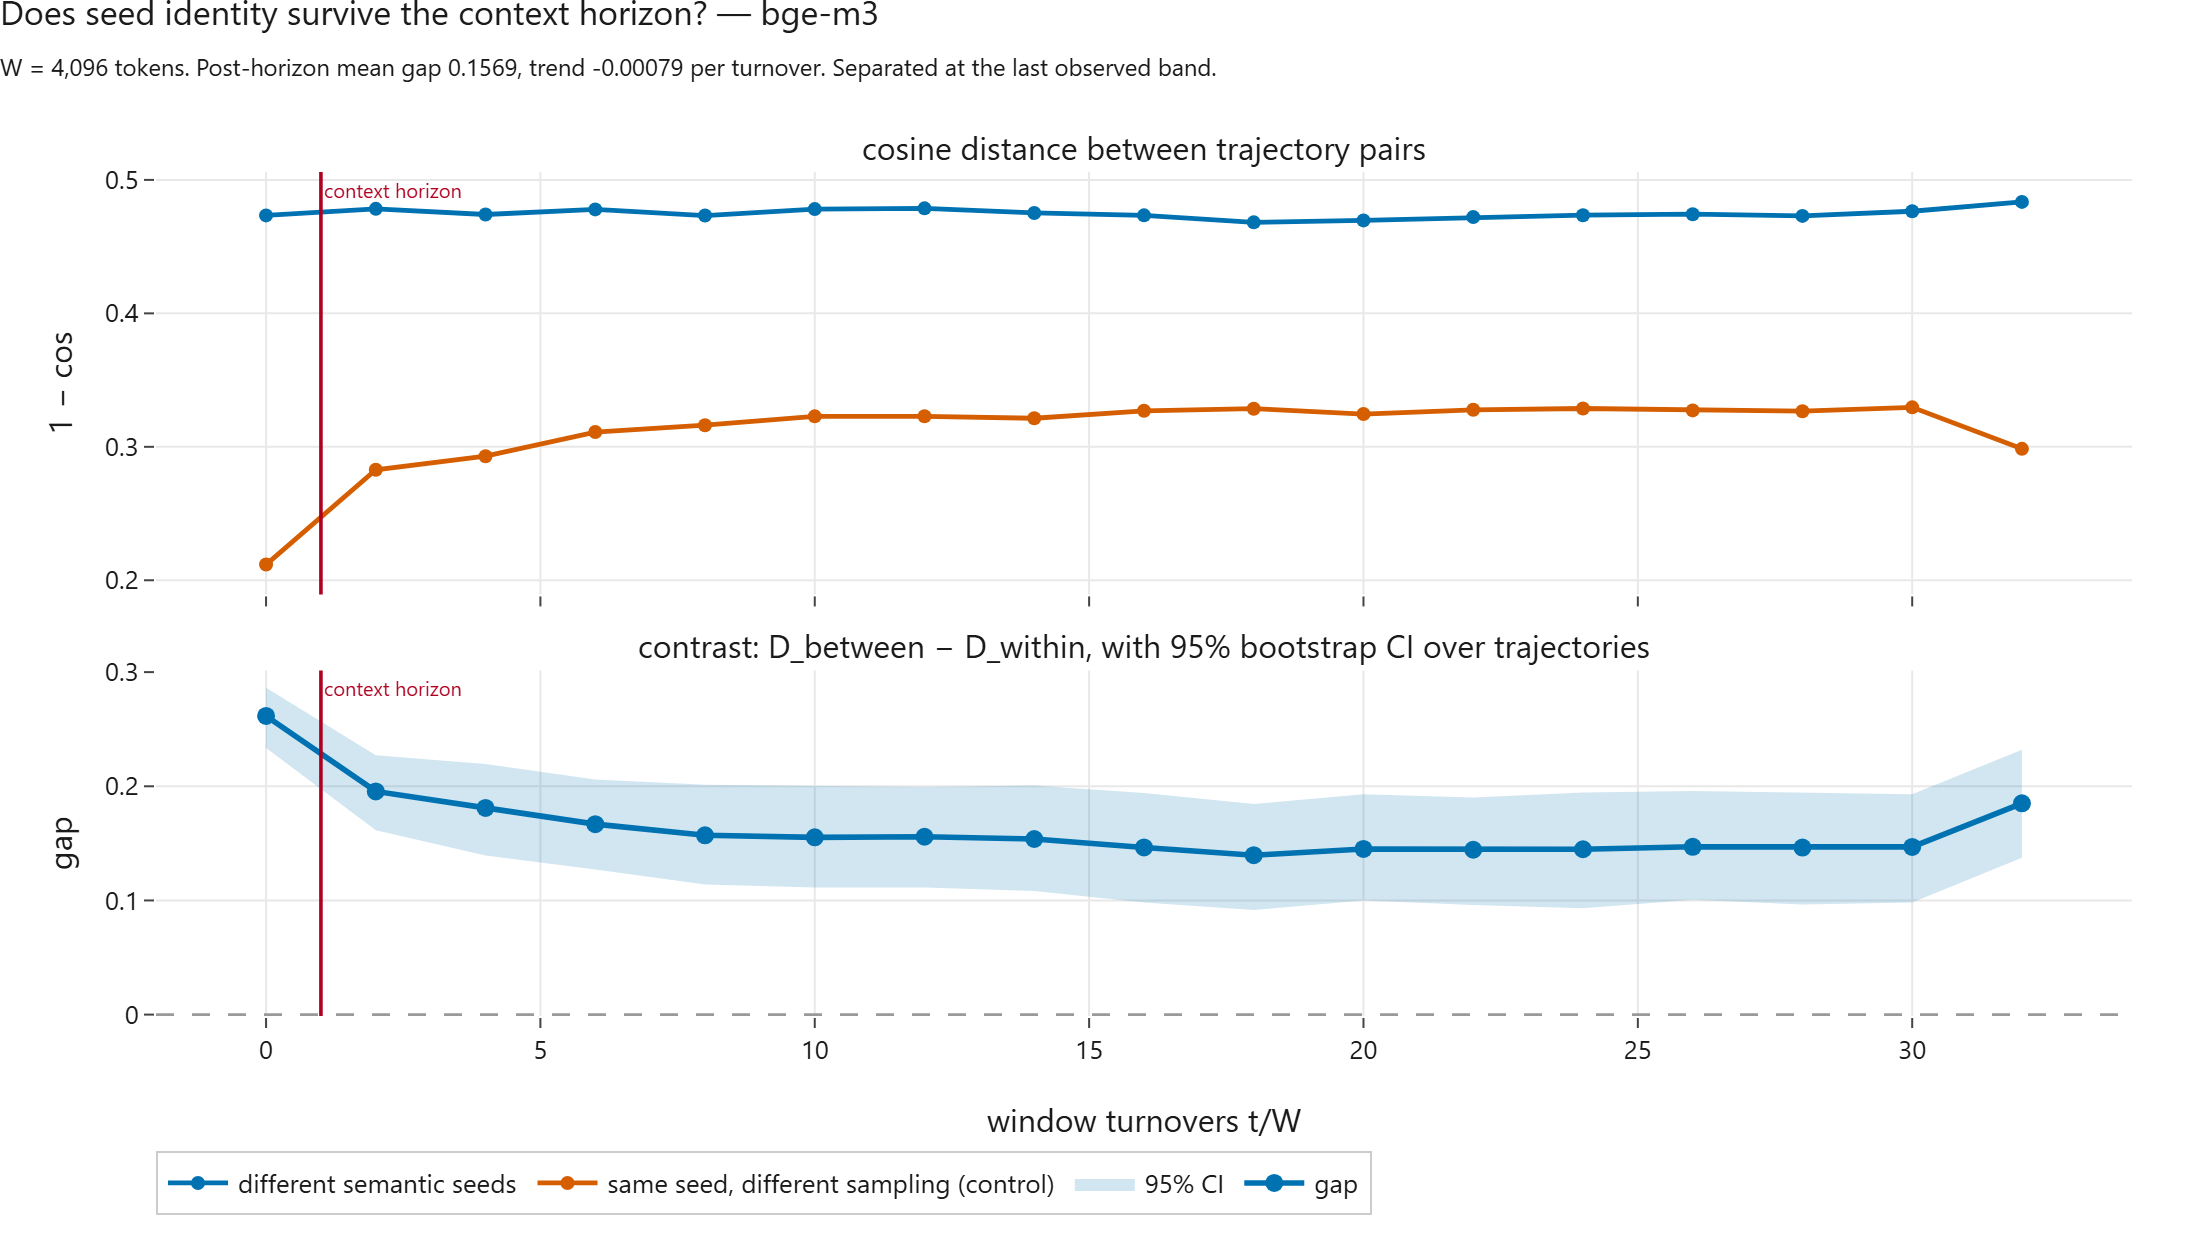
\includegraphics[width=0.92\linewidth]{stage-1/separation-bge-m3/seed_separation.png}
  \caption{Stage~1 domain-gap versus turnover in \texttt{bge-m3} on the
    $48$-trajectory \texttt{or-qwen3-8b} pilot. The curve is compatible with % artifacts/stage-1/separation-bge-m3/seed_separation.png @ s1-separation-bge-m3-20260831T074042Z-9bf54fbf
    seed-family identity surviving the horizon on this degenerate-majority
    panel. It is not a claim that the same gap exists in a non-looping
    subsample, at another generator, or under a sliding KV cache.
    Data: \texttt{artifacts/stage-1/separation-bge-m3/seed\_separation.data.parquet}.
    Generate: \texttt{s1-pilot-core-20260830T134147Z-f1cce9ec}.
    Embed: \texttt{s1-embed-pilot-core-20260831T064430Z-f05e6a68}.
    Separation: \texttt{s1-separation-bge-m3-20260831T074042Z-9bf54fbf}.} % artifacts/stage-1/separation-bge-m3/seed_separation.png @ s1-separation-bge-m3-20260831T074042Z-9bf54fbf
  \label{fig:s1-sep}
\end{figure}

\subsection{Stage 2: the lock is not universal across hosted generators}
\label{sec:s2}

Table~\ref{tab:s2-rates} reports textual-fixed-point rates on a four-model
axis at $T{=}0.3$, $W{=}4096$. % artifacts/stage-2/model-axis/rates/fixed_point_rates.csv @ s2-rates-20260901T125506Z-41d2e88e
\texttt{or-gemma-4-31b} is $0/8$ (CI $[0,0]$). % artifacts/stage-2/model-axis/rates/fixed_point_rates.csv @ s2-rates-20260901T125506Z-41d2e88e
\texttt{or-gpt-oss-120b} is $8/8$ (CI $[1,1]$), under an almost-$T$ caveat % artifacts/stage-2/model-axis/rates/fixed_point_rates.csv @ s2-rates-20260901T125506Z-41d2e88e
documented in the Stage~2 report. % artifacts/stage-2/model-axis/rates/fixed_point_rates.csv @ s2-rates-20260901T125506Z-41d2e88e
\texttt{or-muse-glimmer-30b} is $2/8$ (CI $[0, 0.625]$); the rates file % artifacts/stage-2/model-axis/rates/fixed_point_rates.csv @ s2-model-axis-20260901T015457Z-ab59afc8
counts incomplete trajectories, and only the two long physics cells reached
target $T$. % artifacts/stage-2/model-axis/rates/fixed_point_rates.csv @ s2-model-axis-20260901T015457Z-ab59afc8
\texttt{or-qwen3-8b} on this arm is $7/8$ (CI $[0.625, 1]$). % artifacts/stage-2/model-axis/rates/fixed_point_rates.csv @ s2-rates-20260901T125506Z-41d2e88e
\texttt{or-gpt-oss-20b} contributed $0/8$ trajectories that reached target % docs/stages/stage-2/REPORT.md @ s2-model-axis-20260901T015457Z-ab59afc8
$T$ (empty-EOS deaths); the rates CSV's $2/7$ is not used. % docs/stages/stage-2/REPORT.md @ s2-model-axis-20260901T015457Z-ab59afc8
Across the model-axis file, $11/40$ trajectories reached target $T$. % docs/stages/stage-2/REPORT.md @ s2-model-axis-20260901T015457Z-ab59afc8

A prefill-versus-raw mechanism arm on \texttt{or-qwen3-8b} did not detect a
prefill-driven change in the lock rate: $7/8$ versus $8/8$, difference CI % docs/stages/stage-2/REPORT.md @ s2-mechanism-20260901T071519Z-dfbb173a
$[-0.375, 0]$. % docs/stages/stage-2/REPORT.md @ s2-mechanism-20260901T071519Z-dfbb173a
Provider determinism, measured as exact text match on a short probe, was
$100\%$ (\texttt{or-muse-glimmer-30b}), $60\%$ (\texttt{or-qwen3-8b}), $20\%$ % docs/stages/stage-2/REPORT.md @ s2-audit-determinism-20260901T015221Z-ab59afc8
(\texttt{or-gemma-4-31b}), and $20\%$ (\texttt{or-gpt-oss-120b}). % docs/stages/stage-2/REPORT.md @ s2-audit-determinism-20260901T015221Z-ab59afc8
The occupancy stages therefore cannot treat replica pairs as independent
draws from a deterministic decoder.

The Stage~2 rate figure exists only as SVG
(\texttt{artifacts/stage-2/model-axis/rates/fixed\_point\_rate.svg}). % artifacts/stage-2/model-axis/rates/fixed_point_rate.svg @ s2-rates-20260901T125506Z-41d2e88e
This manuscript uses the CSV table rather than a rasterised substitute.

\begin{table}[t]
  \centering
  \caption{Textual fixed-point rates, Stage~2 model axis, $T{=}0.3$,
    $W{=}4096$. Source:
    \texttt{artifacts/stage-2/model-axis/rates/fixed\_point\_rates.csv};
    \texttt{s2-rates-20260901T125506Z-41d2e88e}.
    Gemma's $0/8$ is the existence proof that the Stage~1 freeze is not a % artifacts/stage-2/model-axis/rates/fixed_point_rates.csv @ s2-rates-20260901T125506Z-41d2e88e
    property of instruct models as a class.} % artifacts/stage-2/model-axis/rates/fixed_point_rates.csv @ s2-rates-20260901T125506Z-41d2e88e
  \label{tab:s2-rates}
  \begin{tabular}{@{}lccc@{}}
    \toprule
    Generator & $n$ in rates file & fixed-point rate & 95\% CI \\
    \midrule
    \texttt{or-qwen3-8b} & $8$ & $7/8$ & $[0.625, 1]$ \\ % artifacts/stage-2/model-axis/rates/fixed_point_rates.csv @ s2-rates-20260901T125506Z-41d2e88e
    \texttt{or-gemma-4-31b} & $8$ & $0/8$ & $[0, 0]$ \\ % artifacts/stage-2/model-axis/rates/fixed_point_rates.csv @ s2-rates-20260901T125506Z-41d2e88e
    \texttt{or-gpt-oss-120b} & $8$ & $8/8$ & $[1, 1]$ \\ % artifacts/stage-2/model-axis/rates/fixed_point_rates.csv @ s2-rates-20260901T125506Z-41d2e88e
    \texttt{or-muse-glimmer-30b} & $8$ & $2/8$ & $[0, 0.625]$ \\ % artifacts/stage-2/model-axis/rates/fixed_point_rates.csv @ s2-rates-20260901T125506Z-41d2e88e
    \texttt{or-gpt-oss-20b} & $0$ reached $T$ & --- & --- \\ % docs/stages/stage-2/REPORT.md @ s2-model-axis-20260901T015457Z-ab59afc8
    \bottomrule
  \end{tabular}
\end{table}

\subsection{Stage 3: no validated MSM; $n_{\mathrm{macro}}$ is not an order parameter}
\label{sec:s3}

Stage~3 applied VAMP/PCCA+ on embeddings of the Stage~1 panel and a local-base
probe. The validation table is uniformly negative:
\texttt{validated=0} in every cell of
\texttt{artifacts/stage-3/dynamics/k\_stability.md}. % artifacts/stage-3/dynamics/k_stability.md @ s3-dynamics-20260901T204521Z-f21d5908
Implied $n_{\mathrm{macro}}$ is unstable across $K$ and across embedding
spaces. Microstate Chapman--Kolmogorov tests fail a $0.15$ bar. % artifacts/stage-3/dynamics/k_stability.md @ s3-dynamics-20260901T204549Z-b7c4d0c9
Hypothesis H1 (metastable semantic states as an MSM object) is unsupported.
The Frobenius norm of a probability current computed on \emph{microstates}
is not evidence for H4 (non-reversible currents among macrostates).

A local \texttt{gemma-3-1b-pt} probe at $W{=}256$ produced $8/8$ degenerate % docs/stages/stage-3/REPORT.md @ s3-local-base-20260901T184812Z-cc80633b
trajectories and $0/8$ reviewer-register rows. % docs/stages/stage-3/REPORT.md @ s3-local-base-20260901T184812Z-cc80633b
That cell is a different window from the occupancy panel. It does not fill
the missing hosted-base cell from Stage~0, and it does not license a
base-versus-instruct claim at $W{=}4096$.

\subsection{Stage 4: lock until $T{=}1.5$; H5 is absent} % artifacts/stage-4/grid/looping_rate_by_cell.csv @ s4-w4096-new-temps-20260904T103121Z-589c8eb1
\label{sec:s4}

Stage~4 crossed temperature and window on \texttt{or-qwen3-8b} with $n{=}4$
trajectories per cell. % artifacts/stage-4/grid/looping_rate_by_cell.csv @ s4-w4096-new-temps-20260904T103121Z-589c8eb1
Table~\ref{tab:s4-loop} summarises looping rates. At $T \le 1.0$, both
$W{=}4096$ and $W{=}8192$ are $4/4$ looping (CI $[1,1]$). % artifacts/stage-4/grid/looping_rate_by_cell.csv @ s4-w4096-new-temps-20260904T103121Z-589c8eb1
At $T{=}1.5$, $W{=}4096$ is $0/4$ looping (CI $[0,0]$); $W{=}8192$ is $2/4$ (CI $[0,1]$). % artifacts/stage-4/grid/looping_rate_by_cell.csv @ s4-w8192-20260904T120057Z-ce82ce55

Clean MSD $\alpha$ is defined only in cells that are not looping.
The defined cells are $T{=}1.5$: at $W{=}4096$, $\alpha = 0.149$ $[0.140, 0.158]$ in % artifacts/stage-4/grid/clean_alpha_by_cell.csv @ s4-w4096-new-temps-20260904T103121Z-589c8eb1
\texttt{bge-m3} and $\alpha = 0.277$ $[0.241, 0.318]$ in % artifacts/stage-4/grid/clean_alpha_by_cell.csv @ s4-w4096-new-temps-20260904T103121Z-589c8eb1
\texttt{qwen3-embed-8b}; % artifacts/stage-4/grid/clean_alpha_by_cell.csv @ s4-w4096-new-temps-20260904T103121Z-589c8eb1
at $W{=}8192$ ($n_{\mathrm{clean}}{=}2$), $\alpha = 0.146$ $[0.086, 0.207]$ in % artifacts/stage-4/grid/clean_alpha_by_cell.csv @ s4-w8192-20260904T120057Z-ce82ce55
\texttt{bge-m3} and $\alpha = 0.247$ $[0.172, 0.322]$ in % artifacts/stage-4/grid/clean_alpha_by_cell.csv @ s4-w8192-20260904T120057Z-ce82ce55
\texttt{qwen3-embed-8b}. % artifacts/stage-4/grid/clean_alpha_by_cell.csv @ s4-w8192-20260904T120057Z-ce82ce55
All four estimates are subdiffusive. There is no low-$T$ clean $\alpha$, so H5
(non-looping confined motion in a temperature window) is absent, not
borderline. Figure~\ref{fig:s4-loop} and Figure~\ref{fig:s4-alpha} are the
committed Stage~4 figures. $n{=}4$ is the whole cell, not a large-sample
rate.

\begin{table}[t]
  \centering
  \caption{Looping rate by temperature and window, Stage~4,
    \texttt{or-qwen3-8b}, $n{=}4$ per cell. Source:
    \texttt{artifacts/stage-4/grid/looping\_rate\_by\_cell.csv}.
    Degeneracy thresholds remain Jaccard $0.083$ / late $0.0122$.} % artifacts/stage-1/degeneracy/degeneracy_verdicts.meta.json @ s1-degeneracy-20260831T070038Z-b2f6f0c9
  \label{tab:s4-loop}
  \begin{tabular}{@{}lcccc@{}}
    \toprule
    $T$ & $W{=}4096$ looping & CI & $W{=}8192$ looping & CI \\
    \midrule
    $\le 1.0$ & $4/4$ & $[1,1]$ & $4/4$ & $[1,1]$ \\ % artifacts/stage-4/grid/looping_rate_by_cell.csv @ s4-w4096-new-temps-20260904T103121Z-589c8eb1
    $1.5$ & $0/4$ & $[0,0]$ & $2/4$ & $[0,1]$ \\ % artifacts/stage-4/grid/looping_rate_by_cell.csv @ s4-w8192-20260904T120057Z-ce82ce55
    \bottomrule
  \end{tabular}
\end{table}

\begin{figure}[t]
  \centering
  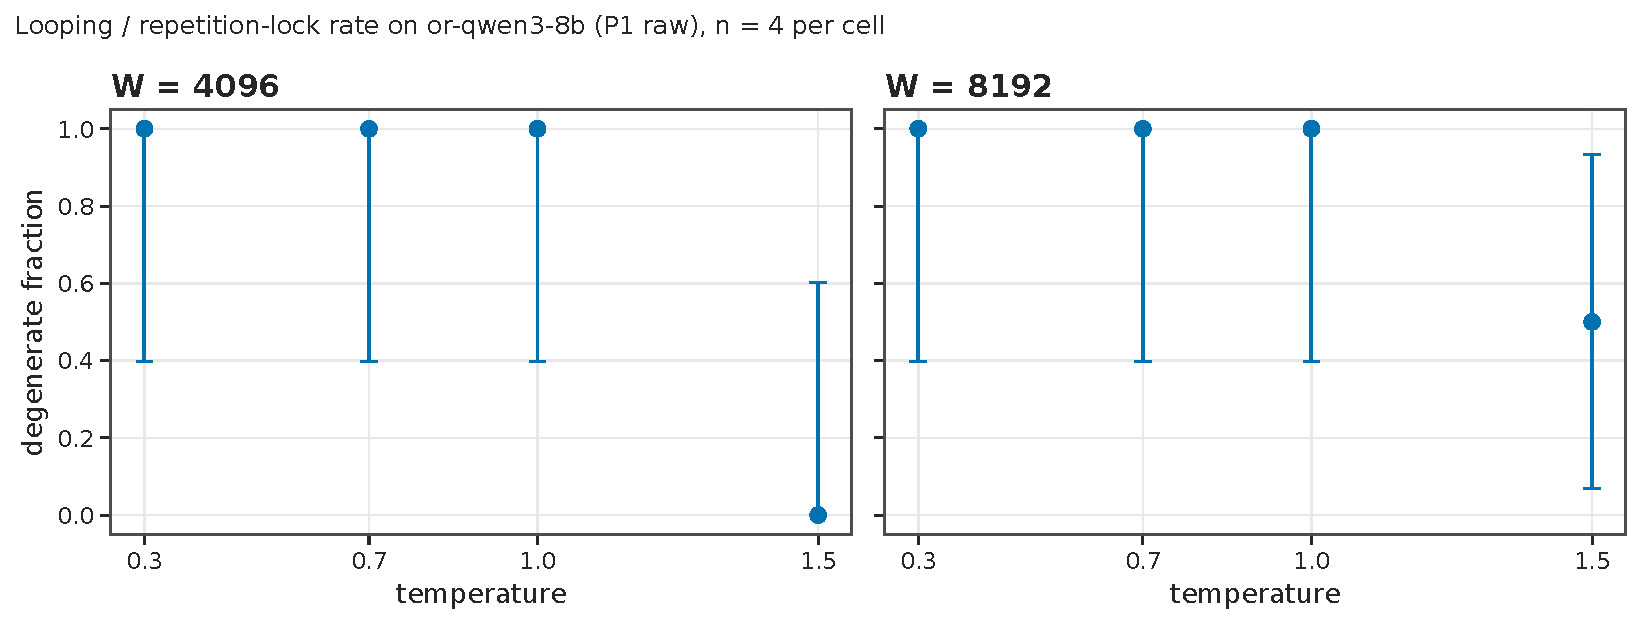
\includegraphics[width=0.85\linewidth]{stage-4/grid/looping_rate_vs_T.pdf}
  \caption{Looping rate versus temperature at two windows.
    Data: \texttt{artifacts/stage-4/grid/looping\_rate\_vs\_T.data.parquet}.
    Generate: \texttt{s4-w4096-new-temps-20260904T103121Z-589c8eb1},
    \texttt{s4-w8192-20260904T120057Z-ce82ce55}.
    The $T{=}1.5$, $W{=}4096$ cell is the existence of a non-looping regime % artifacts/stage-4/grid/looping_rate_vs_T.pdf @ s4-w4096-new-temps-20260904T103121Z-589c8eb1
    on this model, not a mixing-time estimate.} % artifacts/stage-4/grid/looping_rate_vs_T.pdf @ s4-w4096-new-temps-20260904T103121Z-589c8eb1
  \label{fig:s4-loop}
\end{figure}

\begin{figure}[t]
  \centering
  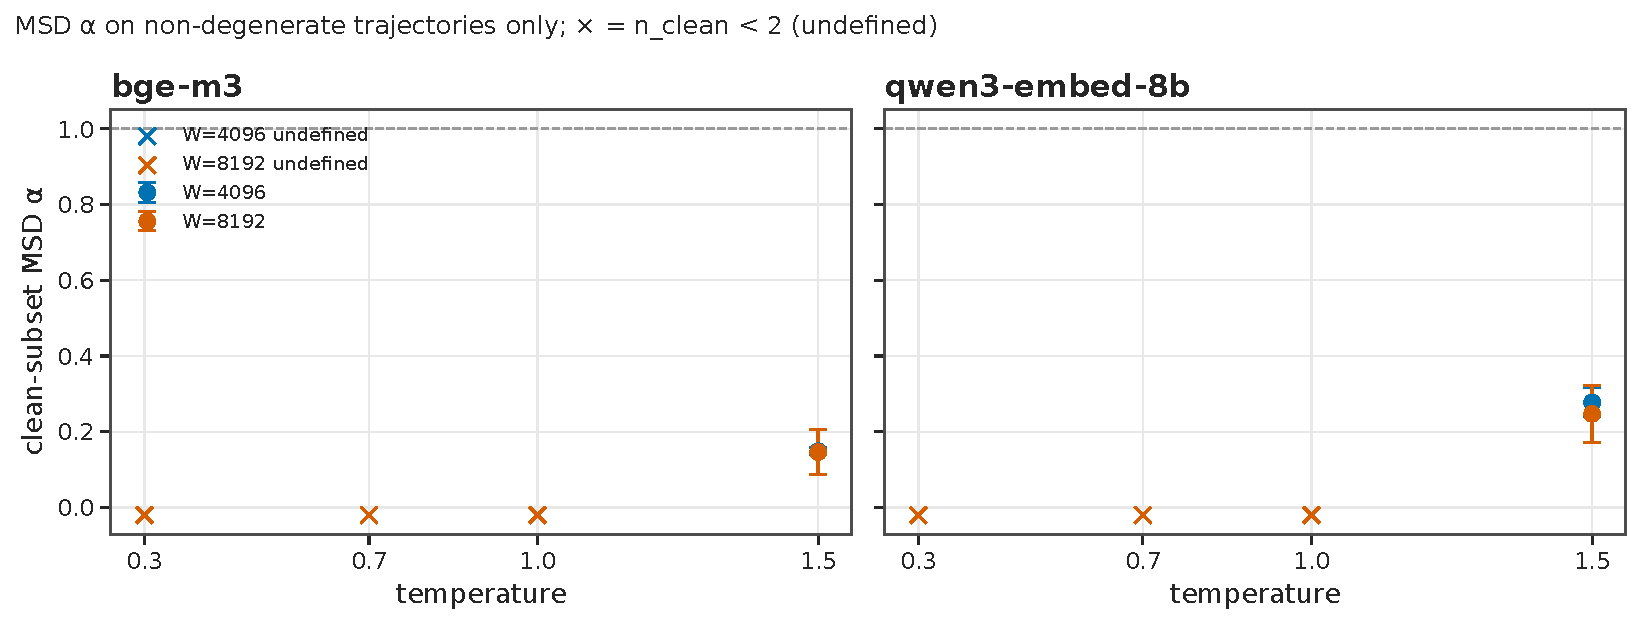
\includegraphics[width=0.85\linewidth]{stage-4/grid/clean_alpha_vs_T.pdf}
  \caption{Clean MSD $\alpha$ where defined (non-looping cells only).
    Data: \texttt{artifacts/stage-4/grid/clean\_alpha\_vs\_T.data.parquet}.
    Missing low-$T$ points are the H5 absence, not a plotting omission.} % artifacts/stage-4/grid/clean_alpha_vs_T.pdf @ s4-w4096-new-temps-20260904T103121Z-589c8eb1
  \label{fig:s4-alpha}
\end{figure}

\subsection{Stage 5: last-band occupancy on the locked panel}
\label{sec:s5}

Given the lock, Stage~5 asks two occupancy questions on twenty-eight
\texttt{or-qwen3-8b} trajectories at $W{=}4096$, $T{=}0.3$, twelve turnovers. % docs/stages/stage-5/REPORT.md @ s5-lock-occupancy-20260905T164327Z-6780902f
Generate \texttt{s5-lock-occupancy-20260905T164327Z-6780902f};
embed \texttt{s5-embed-lock-occupancy-20260906T030125Z-eab6e484};
degeneracy \texttt{s5-degeneracy-20260906T030145Z-deb4c3bd}.
Ten domain seeds (including love) contribute two replicas each; four twin
seeds contribute the F6 pairs.

Lock occupancy: $19/20$ domain trajectories and $10/10$ domain seeds meet % artifacts/stage-5/occupancy/lock_rate_by_seed.csv @ s5-degeneracy-20260906T030145Z-deb4c3bd
the textual-fixed-point rule; love is $1/2$. % artifacts/stage-5/occupancy/lock_rate_by_seed.csv @ s5-degeneracy-20260906T030145Z-deb4c3bd

F4 in two spaces, last band, ten domain seeds, $n{=}20$ trajectories,
$n_{\mathrm{within}}{=}9$ pairs after physics seed~1 drops from the last-band % artifacts/stage-5/occupancy/domain_separation_last_band.csv @ s5-lock-occupancy-20260905T164327Z-6780902f
diagonal:
\texttt{bge-m3} gap $0.201$, 95\% CI $[0.065, 0.332]$, separated; % artifacts/stage-5/occupancy/domain_separation_last_band.csv @ s5-lock-occupancy-20260905T164327Z-6780902f
\texttt{qwen3-embed-8b} gap $0.390$, CI $[0.151, 0.593]$, separated. % artifacts/stage-5/occupancy/domain_separation_last_band.csv @ s5-lock-occupancy-20260905T164327Z-6780902f
That last-band gap is ensemble distinguishability, not recovered prompt
memory (H2).
Figure~\ref{fig:s5-dom} shows the gap versus turnover in those two spaces.

F6 (replica $\Delta$): every last-band CI includes $0$ on this panel. % artifacts/stage-5/occupancy/twin_last_band.csv @ s5-lock-occupancy-20260905T164327Z-6780902f
Operational collapsed is that CI statement. It is not occupancy of one lock.
The Waterloo pair in \texttt{bge-m3} has a last-band point estimate near
$0.049$ whose CI still includes $0$. % artifacts/stage-5/occupancy/twin_last_band.csv @ s5-lock-occupancy-20260905T164327Z-6780902f
The Stage~5 twin-$\Delta$ figure is SVG-only; the three-space figure in
Section~\ref{sec:s6} supersedes it for the manuscript.

\begin{figure}[t]
  \centering
  
\includegraphics[width=0.92\linewidth]{stage-5/occupancy/domain_separation_vs_turnover.pdf}
  \caption{Domain gap versus turnover in \texttt{bge-m3} and
    \texttt{qwen3-embed-8b} on the Stage~5 locked panel. Last-band CIs
    exclude $0$ from above in both spaces. The figure does not include % artifacts/stage-5/occupancy/domain_separation_vs_turnover.pdf @ s5-lock-occupancy-20260905T164327Z-6780902f
    \texttt{gemini-embed-001} (Stage~6) and does not show a non-looping
    subsample.
    Data: \texttt{artifacts/stage-5/occupancy/domain\_separation\_vs\_turnover.data.parquet}.
    Generate: \texttt{s5-lock-occupancy-20260905T164327Z-6780902f}.} % artifacts/stage-5/occupancy/domain_separation_vs_turnover.pdf @ s5-lock-occupancy-20260905T164327Z-6780902f
  \label{fig:s5-dom}
\end{figure}

\subsection{Stage 6: occupancy signs in a third embedding space}
\label{sec:s6}

Stage~6 re-embedded the same $28$ trajectories in % docs/stages/stage-6/REPORT.md @ s6-embed-third-space-20260906T082301Z-588eff8f
\texttt{gemini-embed-001} and reassembled F4/F6 in three spaces. No new
tokens were generated. Hosted Stage~6 spend is $\$0$. % docs/stages/stage-6/REPORT.md @ s6-embed-third-space-20260906T082301Z-588eff8f
Gemini embedding runs:
\texttt{s6-embed-third-space-20260906T082301Z-588eff8f},
\texttt{s6-embed-third-space-20260906T082628Z-9077d587}.

Table~\ref{tab:s6-f4} reports last-band F4. All three spaces are
\texttt{separated} under the pre-registered CI rule. The gemini interval
$[0.029, 0.266]$ excludes $0$ by a whisker. % artifacts/stage-6/occupancy/domain_separation_last_band.csv @ s6-embed-third-space-20260906T082301Z-588eff8f
That is an NHST pass, not
thick robustness, and not architecture-independence. The three spaces
disagree on \emph{level}: $0.201$ / $0.390$ / $0.150$. % artifacts/stage-6/occupancy/domain_separation_last_band.csv @ s6-embed-third-space-20260906T082301Z-588eff8f
Sign agreement is the claim. Physics seed~1 has $47$ versus $48$ chunks, so % docs/stages/stage-6/REPORT.md @ s6-embed-third-space-20260906T082301Z-588eff8f
its last-band $D_{\mathrm{within}}$ diagonal is undefined (NaN) in every
space; F4 uses the remaining $n_{\mathrm{within}}{=}9$ pairs. % docs/stages/stage-6/REPORT.md @ s6-embed-third-space-20260906T082301Z-588eff8f

Table~\ref{tab:s6-f6} reports last-band F6. Gemini all-pairs $\Delta$ is
$-0.012$, CI $[-0.286, 0.223]$ (includes $0$). % artifacts/stage-6/occupancy/twin_last_band.csv @ s6-embed-third-space-20260906T082301Z-588eff8f
The reactor pair never excluded $0$ in any space % artifacts/stage-6/occupancy/twin_last_band.csv @ s6-embed-third-space-20260906T082301Z-588eff8f
($0.008$, CI $[-0.071, 0.087]$ in gemini). % artifacts/stage-6/occupancy/twin_last_band.csv @ s6-embed-third-space-20260906T082301Z-588eff8f
Waterloo gemini last-band $\Delta$ is $-0.031$, CI $[-0.286, 0.223]$; % artifacts/stage-6/occupancy/twin_per_band.csv @ s6-embed-third-space-20260906T082301Z-588eff8f
the same pair at band $0$ is $0.033$, CI $[0.001, 0.065]$, so the sign % artifacts/stage-6/occupancy/twin_per_band.csv @ s6-embed-third-space-20260906T082301Z-588eff8f
flips along the trajectory. % artifacts/stage-6/occupancy/twin_per_band.csv @ s6-embed-third-space-20260906T082301Z-588eff8f
Operational collapsed remains ``CI includes $0$'', not ``the two replicas % artifacts/stage-6/occupancy/twin_per_band.csv @ s6-embed-third-space-20260906T082301Z-588eff8f
occupy one lock''.

Figure~\ref{fig:s6-f4} and Figure~\ref{fig:s6-f6} are the Stage~6
three-space figures. Figure~\ref{fig:s6-heat} is a last-band cosine-distance
matrix in gemini space. It is an illustration of pairwise distances, not a
cluster count, and not a 2-D projection used as evidence.

A protocol diagnostic on the same panel, not a headline result: domain
trajectories spend a mean fill fraction $0.853$, 95\% CI $[0.756, 0.936]$, % artifacts/stage-5/occupancy/protocol_by_quarter.csv @ s5-lock-occupancy-20260905T164327Z-6780902f
in the last quarter, with mean stop-token fraction $0.359$. % artifacts/stage-5/occupancy/protocol_by_quarter.csv @ s5-lock-occupancy-20260905T164327Z-6780902f
P1 fill is a confound to name, not a sliding-window measurement.

\begin{table}[t]
  \centering
  \caption{F4 last-band domain gap, ten domain seeds, $n{=}20$,
    $n_{\mathrm{within}}{=}9$. Source: % CI excludes $0$ from above.} % artifacts/stage-6/occupancy/domain_separation_last_band.csv @ s6-embed-third-space-20260906T082301Z-588eff8f
    \texttt{artifacts/stage-6/occupancy/domain\_separation\_last\_band.csv}.
    Generate: \texttt{s5-lock-occupancy-20260905T164327Z-6780902f}.
    Gemini embeds: \texttt{s6-embed-third-space-20260906T082301Z-588eff8f},
    \texttt{s6-embed-third-space-20260906T082628Z-9077d587}.
    Separated means the 95\% CI excludes $0$ from above.} % artifacts/stage-6/occupancy/domain_separation_last_band.csv @ s6-embed-third-space-20260906T082301Z-588eff8f
  \label{tab:s6-f4}
  \begin{tabular}{@{}lccc@{}}
    \toprule
    Space & gap & 95\% CI & separated \\
    \midrule
    \texttt{bge-m3} & $0.201$ & $[0.065, 0.332]$ & yes \\ % artifacts/stage-6/occupancy/domain_separation_last_band.csv @ s5-lock-occupancy-20260905T164327Z-6780902f
    \texttt{qwen3-embed-8b} & $0.390$ & $[0.151, 0.593]$ & yes \\ % artifacts/stage-6/occupancy/domain_separation_last_band.csv @ s5-lock-occupancy-20260905T164327Z-6780902f
    \texttt{gemini-embed-001} & $0.150$ & $[0.029, 0.266]$ & yes \\ % artifacts/stage-6/occupancy/domain_separation_last_band.csv @ s6-embed-third-space-20260906T082301Z-588eff8f
    \bottomrule
  \end{tabular}
\end{table}

\begin{table}[t]
  \centering
  \caption{F6 last-band replica $\Delta$, operational collapsed $=$ CI
    includes $0$. Source: % artifacts/stage-6/occupancy/twin_last_band.csv @ s6-embed-third-space-20260906T082301Z-588eff8f
    \texttt{artifacts/stage-6/occupancy/twin\_last\_band.csv}.
    This table is not occupancy of one lock.} % artifacts/stage-6/occupancy/twin_last_band.csv @ s6-embed-third-space-20260906T082301Z-588eff8f
  \label{tab:s6-f6}
  \begin{tabular}{@{}lccc@{}}
    \toprule
    Slice & $\Delta$ & 95\% CI & CI includes $0$ \\
    \midrule
    gemini, all pairs & $-0.012$ & $[-0.286, 0.223]$ & yes \\ % artifacts/stage-6/occupancy/twin_last_band.csv @ s6-embed-third-space-20260906T082301Z-588eff8f
    reactor, gemini & $0.008$ & $[-0.071, 0.087]$ & yes \\ % artifacts/stage-6/occupancy/twin_last_band.csv @ s6-embed-third-space-20260906T082301Z-588eff8f
    waterloo, gemini last band & $-0.031$ & $[-0.286, 0.223]$ & yes \\ % artifacts/stage-6/occupancy/twin_last_band.csv @ s6-embed-third-space-20260906T082301Z-588eff8f
    waterloo, gemini band $0$ & $0.033$ & $[0.001, 0.065]$ & no \\ % artifacts/stage-6/occupancy/twin_per_band.csv @ s6-embed-third-space-20260906T082301Z-588eff8f
    \bottomrule
  \end{tabular}
\end{table}

\begin{figure}[t]
  \centering
  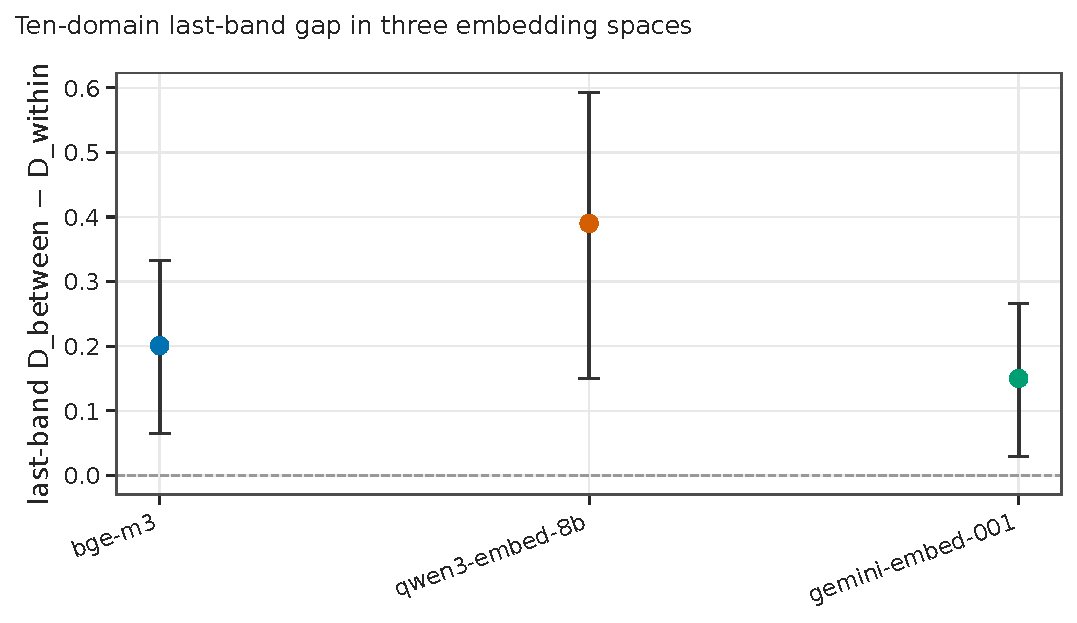
\includegraphics[width=0.92\linewidth]{stage-6/occupancy/domain_gap_three_spaces.pdf}
  \caption{F4 domain gap versus turnover in three embedding spaces on the
    same $28$ \texttt{or-qwen3-8b} trajectories. Last-band CIs exclude $0$ % artifacts/stage-6/occupancy/domain_gap_three_spaces.pdf @ s6-embed-third-space-20260906T082301Z-588eff8f
    in all three spaces; gemini is the whisker. Levels $0.201$ / $0.390$ / % artifacts/stage-6/occupancy/domain_gap_three_spaces.pdf @ s6-embed-third-space-20260906T082301Z-588eff8f
    $0.150$ are not interchangeable. % artifacts/stage-6/occupancy/domain_gap_three_spaces.pdf @ s6-embed-third-space-20260906T082301Z-588eff8f
    Data: \texttt{artifacts/stage-6/occupancy/domain\_gap\_three\_spaces.data.parquet}.} % artifacts/stage-6/occupancy/domain_gap_three_spaces.pdf @ s6-embed-third-space-20260906T082301Z-588eff8f
  \label{fig:s6-f4}
\end{figure}

\begin{figure}[t]
  \centering
  
\includegraphics[width=0.92\linewidth]{stage-6/occupancy/twin_delta_vs_turnover.pdf}
  \caption{F6 replica $\Delta$ versus turnover in three spaces.
    Last-band CIs include $0$. Waterloo in gemini flips sign from band $0$ % artifacts/stage-6/occupancy/twin_delta_vs_turnover.pdf @ s6-embed-third-space-20260906T082301Z-588eff8f
    to the last band. Operational collapsed is that CI statement, not a
    shared lock.
    Data: \texttt{artifacts/stage-6/occupancy/twin\_delta\_vs\_turnover.data.parquet}.} % artifacts/stage-6/occupancy/twin_delta_vs_turnover.pdf @ s6-embed-third-space-20260906T082301Z-588eff8f
  \label{fig:s6-f6}
\end{figure}

\begin{figure}[t]
  \centering
  
\includegraphics[width=0.72\linewidth]{stage-6/occupancy/last_band_distance_matrix_gemini_embed_001.pdf}
  \caption{Last-band cosine distances in \texttt{gemini-embed-001}
    (illustration of the pairwise matrix, not a cluster count, not a 2-D
    projection). Physics seed~1 is the incomplete last band.
    Data: \texttt{artifacts/stage-6/occupancy/last\_band\_distance\_matrix\_gemini\_embed\_001.data.parquet}.} % artifacts/stage-6/occupancy/last_band_distance_matrix_gemini_embed_001.pdf @ s6-embed-third-space-20260906T082301Z-588eff8f
  \label{fig:s6-heat}
\end{figure}

\section{Limitations}
\label{sec:limitations}

\paragraph{P1 versus sliding attention.}
Every afterlife token in this paper is produced by re-prompting the last $W$
tokens. A native sliding KV cache was not measured. ADR-0017 parks that
comparison. No sentence here is evidence about sliding attention.

\paragraph{Representation.}
Occupancy signs agree in \texttt{bge-m3}, \texttt{qwen3-embed-8b}, and
\texttt{gemini-embed-001}. Absolute gaps do not: $0.201$, $0.390$, $0.150$. % artifacts/stage-6/occupancy/domain_separation_last_band.csv @ s6-embed-third-space-20260906T082301Z-588eff8f
Gemini F4 is an NHST whisker ($0.029$ on the lower CI). % artifacts/stage-6/occupancy/domain_separation_last_band.csv @ s6-embed-third-space-20260906T082301Z-588eff8f
That is not
architecture-independence, and Stage~6 closed on that wording. We do not
report ARI/NMI across spaces; the cross-embedding check is F4 sign
agreement.

\paragraph{Provider non-determinism.}
Stage~2 exact-match rates were $100/60/20/20$ percent across four hosted % docs/stages/stage-2/REPORT.md @ s2-audit-determinism-20260901T015221Z-ab59afc8
generators. % docs/stages/stage-2/REPORT.md @ s2-audit-determinism-20260901T015221Z-ab59afc8
Replica pairs on \texttt{or-qwen3-8b} are not guaranteed independent
deterministic draws.

\paragraph{Finite horizon.}
Occupancy uses twelve turnovers, not an infinite afterlife. % docs/stages/stage-5/REPORT.md @ s5-lock-occupancy-20260905T164327Z-6780902f
Stage~1 reached
$32$ turnovers on a different seed panel; that length is not reused as an % docs/stages/stage-1/REPORT.md @ s1-pilot-core-20260830T134147Z-f1cce9ec
occupancy mixing time. % docs/stages/stage-1/REPORT.md @ s1-pilot-core-20260830T134147Z-f1cce9ec

\paragraph{Metastability versus lock.}
A textual fixed point is a lock in token space. It is not a validated MSM
macrostate. Stage~3 found \texttt{validated=0} in every cell. % artifacts/stage-3/dynamics/k_stability.md @ s3-dynamics-20260901T204521Z-f21d5908
This paper does not use ``metastable semantic states'' as an established
finding.

\paragraph{One generator, one protocol, one temperature for occupancy.}
F4 and F6 are \texttt{or-qwen3-8b}, P1, \texttt{raw\_completion}, served
provider \texttt{Alibaba}, $T{=}0.3$, $W{=}4096$. % docs/stages/stage-5/REPORT.md @ s5-lock-occupancy-20260905T164327Z-6780902f
P1 is the re-prompt axis; \texttt{raw\_completion} is the continuation
mechanism. They are not synonyms. Stage~2 already measured prefill versus
raw on this generator ($7/8$ versus $8/8$, difference CI $[-0.375, 0]$); % docs/stages/stage-2/REPORT.md @ s2-mechanism-20260901T071519Z-dfbb173a
that arm is not the occupancy protocol. % docs/stages/stage-2/REPORT.md @ s2-mechanism-20260901T071519Z-dfbb173a
Stage~2 already shows a generator where the lock rate is $0/8$. % artifacts/stage-2/model-axis/rates/fixed_point_rates.csv @ s2-rates-20260901T125506Z-41d2e88e
Stage~4 already shows $T{=}1.5$, $W{=}4096$ with $0/4$ looping. % artifacts/stage-4/grid/looping_rate_by_cell.csv @ s4-w4096-new-temps-20260904T103121Z-589c8eb1
Those cells are not occupancy measurements.

\paragraph{Replica $n{=}2$.}
Each domain seed has two trajectories. F6 CIs are wide. A CI that includes
$0$ can be an underpowered non-detection. % artifacts/stage-6/occupancy/domain_separation_last_band.csv @ s6-embed-third-space-20260906T082301Z-588eff8f

\paragraph{F4 whisker and physics seed~1.}
Gemini last-band F4 lower CI is $0.029$. % artifacts/stage-6/occupancy/domain_separation_last_band.csv @ s6-embed-third-space-20260906T082301Z-588eff8f
Physics seed~1 last-band
$D_{\mathrm{within}}$ is NaN because of a $47$ versus $48$ chunk mismatch. % docs/stages/stage-6/REPORT.md @ s6-embed-third-space-20260906T082301Z-588eff8f

\paragraph{F6 is not one lock.}
Operational collapsed means the last-band $\Delta$ CI includes $0$. % artifacts/stage-6/occupancy/twin_per_band.csv @ s6-embed-third-space-20260906T082301Z-588eff8f
Waterloo in gemini flips sign from band $0$ ($0.033$, CI excludes $0$) to % artifacts/stage-6/occupancy/twin_per_band.csv @ s6-embed-third-space-20260906T082301Z-588eff8f
the last band ($-0.031$, CI includes $0$). % artifacts/stage-6/occupancy/twin_per_band.csv @ s6-embed-third-space-20260906T082301Z-588eff8f

\paragraph{Degeneracy is the sample.}
$19/20$ domain trajectories are textual fixed points. % artifacts/stage-5/occupancy/lock_rate_by_seed.csv @ s5-degeneracy-20260906T030145Z-deb4c3bd
Occupancy is a fact
about locked text, not about a clean subsample that was held out.
Thresholds $0.083$ / $0.0122$ were not moved; love s1 is kept. % artifacts/stage-1/degeneracy/degeneracy_verdicts.meta.json @ s1-degeneracy-20260831T070038Z-b2f6f0c9

\paragraph{No hosted base model.}
Stage~0 found none. The local-base probe is \texttt{gemma-3-1b-pt} at
$W{=}256$, not the occupancy window. % docs/stages/stage-3/REPORT.md @ s3-local-base-20260901T184812Z-cc80633b

\section{Discussion}
\label{sec:discussion}

What is established, on this generator and protocol: after the seed leaves
$W$, the typical $T{=}0.3$ trajectory is a textual lock; last-band centroids
still show an ensemble domain gap across ten seed domains in three embedding
spaces (not recovered prompt memory, H2); replica $\Delta$
CIs at the last band include $0$ and do not justify a one-lock headline. % artifacts/stage-6/occupancy/domain_separation_last_band.csv @ s6-embed-third-space-20260906T082301Z-588eff8f

What is not established: H1 (validated MSM macrostates); H5 (a temperature
window of non-looping confined motion); we cannot claim architecture-independence
of occupancy; a result for language models as a class; P1 versus sliding
attention; mixing times; non-reversible macrostate currents.

\citet{zekri2024} remain the right uniqueness null. Domain-tagged last-band
gaps on a locked panel are compatible with more than one long-run occupancy
region in embedding space. That compatibility is not a proof that the
token-level chain has several stationary measures. It is a measurement of
where locked trajectories sit after twelve turnovers.

The honest next measurement, if any, is not another embedding of the same
$28$ rows. It is a second generator, a sliding-cache contrast, or a % artifacts/stage-6/occupancy/domain_separation_last_band.csv @ s6-embed-third-space-20260906T082301Z-588eff8f
non-looping occupancy panel at $T{=}1.5$. Those are parked, not silently % artifacts/stage-6/occupancy/domain_separation_last_band.csv @ s6-embed-third-space-20260906T082301Z-588eff8f
folded into this manuscript.

\section{Reproducibility}
\label{sec:repro}

Experiments through Stage~6 closed on git commit \texttt{ad1f244}.
A run is \texttt{configs/**} plus that SHA plus a seed. Raw trajectories
live under \texttt{runs/} (gitignored). Publication figures and tidy frames
live under \texttt{artifacts/}. The command
\texttt{afterlife reproduce <run\_id>} is the intended re-derivation path
for a generation or analysis run.

Stage~7 adds this manuscript. It does not add a
\texttt{configs/stages/stage7\_*.yaml} and does not mint a dummy run to
satisfy a generation gate. Hosted Stage~7 spend is $\$0$. % docs/stages/stage-7/REPORT.md @ none

Primary \texttt{run\_id}s cited in the text:

\begin{itemize}
  \item Stage~1 generate: \texttt{s1-pilot-core-20260830T134147Z-f1cce9ec}
  \item Stage~1 degeneracy: \texttt{s1-degeneracy-20260831T070038Z-b2f6f0c9}
  \item Stage~1 embed: \texttt{s1-embed-pilot-core-20260831T064430Z-f05e6a68}
  \item Stage~1 separation: \texttt{s1-separation-bge-m3-20260831T074042Z-9bf54fbf}
  \item Stage~1 geometry: \texttt{s1-geometry-bge-m3-20260831T074420Z-d3c0204a}
  \item Stage~2 model axis: \texttt{s2-model-axis-20260901T015457Z-ab59afc8}
  \item Stage~2 mechanism: \texttt{s2-mechanism-20260901T071519Z-dfbb173a}
  \item Stage~2 determinism: \texttt{s2-audit-determinism-20260901T015221Z-ab59afc8}
  \item Stage~2 rates: \texttt{s2-rates-20260901T125506Z-41d2e88e}
  \item Stage~3 local base: \texttt{s3-local-base-20260901T184812Z-cc80633b}
  \item Stage~3 dynamics: \texttt{s3-dynamics-20260901T204521Z-f21d5908},
        \texttt{s3-dynamics-20260901T204549Z-b7c4d0c9}
  \item Stage~4: \texttt{s4-w4096-new-temps-20260904T103121Z-589c8eb1},
        \texttt{s4-w8192-20260904T120057Z-ce82ce55}
  \item Stage~5 generate: \texttt{s5-lock-occupancy-20260905T164327Z-6780902f}
  \item Stage~5 embed: \texttt{s5-embed-lock-occupancy-20260906T030125Z-eab6e484}
  \item Stage~5 degeneracy: \texttt{s5-degeneracy-20260906T030145Z-deb4c3bd}
  \item Stage~6 gemini: \texttt{s6-embed-third-space-20260906T082301Z-588eff8f},
        \texttt{s6-embed-third-space-20260906T082628Z-9077d587}
\end{itemize}

\bibliographystyle{plainnat}
\bibliography{refs}

\end{document}
